%!TEX root = 3-P_Masterdokument.tex
%!TEX encoding = UTF-8 Unicode

\chapter{Minor word classes}\label{chap:MinorWordClasses}

The major word classes in Paunaka can be considered nouns and verbs, just like in many other languages around the world. They are large and open and described in detail in Chapters \ref{chapter:Nouns} and \ref{sec:Verbs}, respectively.

There are, however, also minor word classes, minor in the sense that they are rather small, with considerably fewer members. Only one of them can be considered absolutely closed, this is the pronouns and nominal demonstratives (§\ref{chapter:Pronouns}). Adpositions can also be considered a fairly closed class (see \sectref{sec:Adpositions}). Among adjectives, numerals, and quantifiers (\sectref{sec:AdjectivesNumerals}), adverbs (\sectref{sec:Adverbs}), and connectives (\sectref{sec:Conjunctions}), however, we find loans\is{borrowing} from Spanish and Bésiro, which shows that these classes are open for new members.


\section{Pronouns and nominal demonstratives}\label{chapter:Pronouns}
\is{pronoun|(}

This section covers pronouns, i.e. personal and topic pronouns, and also nominal demonstratives. It also deals with indefinite pronouns, which occur only rarely in Paunaka discourse. There are personal pronouns for first and second person singular and plural, but not for the third person. (\getref{ex:new23-biti}) includes the first person plural pronoun\is{personal pronoun} \textit{biti}. It comes from Juan Ch. talking about the the different types of work he and the other workers do for their \textit{patrón}.

\ea\label{ex:new23-biti}
\begingl
\glpreamble biti bisu\\
\gla biti bi-isu\\
\glb 1\textsc{pl.prn} 1\textsc{pl}-weed\\
\glft ‘we weed’
\endgl
\trailingcitation{[nxx-p630101g-1.089]}
\xe

In reference to a third person, a topic or demonstrative pronoun\is{nominal demonstrative} can be used instead. Topic pronouns\is{topic pronoun} are used in constructions that involve emphasis, more precisely \isi{topicalisation} (this being reflected in the name chosen for this pronoun) or \isi{focus}. (\getref{ex:new23-chibu}) comes from Miguel.\footnote{Note that this recording has not been archived because it contains sensitive data.}

\ea\label{ex:new23-chibu}
\begingl
\glpreamble chibu tikechunube\\
\gla chibu ti-kechu-nube\\
\glb 3\textsc{top.prn} 3i-say-\textsc{pl}\\
\glft ‘this is what they say’
\endgl
\trailingcitation{[jmx-c120429ls-x5.302]}
\xe

Paunaka has no articles, demonstrative pronouns\is{nominal demonstrative} preceding a noun are predominantly used to mark \isi{definiteness}, as far as I can tell. Nonetheless, just like other pronouns, demonstrative pronoun can occur on their own as well, as in (\getref{ex:new23-echÿu}) from Juana.

\ea\label{ex:new23-echÿu}
\begingl
\glpreamble entonses kuina tamicha echÿu\\
\gla entonses kuina ti-a-micha echÿu\\
\glb thus \textsc{neg} 3i-\textsc{irr}-be.good \textsc{dem}b\\
\glft ‘thus this is not good’
\endgl
\trailingcitation{[jmx-c120429ls-x5.199]}
\xe

There are certain overlaps in the composition of pronouns and nominal demonstratives.\is{nominal demonstrative} These overlaps also include the demonstrative adverbs\is{adverb!demonstrative adverb}\is{demonstrative!demonstrative adverb} and are illustrated in \figref{fig:PronounDemComposition}.

\begin{figure}
\fittable{
\begin{tabular}{|c|c|r|c|l|c|l|}
\multicolumn{1}{c}{Category} & \multicolumn{1}{c}{} & \multicolumn{3}{c}{Composition} & \multicolumn{1}{c}{} & \multicolumn{1}{c}{Rough translation}\cr
\cline{1-1} \cline{3-3} \cline{5-5} \cline{7-7}
\multirow{4}{*}{personal pronouns} && nÿ & + & ti && I\cr
&& pi & + & ti && you (\textsc{sg})\cr
&& bi & + & ti && we\cr
&& e & + & ti && you (\textsc{pl})\cr
\cline{1-1} \cline{5-5}
\multirow{2}{*}{topic pronouns} && chi & + & bu && he, she, it, this\cr
\cline{3-3}
&& ne & + & bu && there\cr
\cline{1-1} \cline{5-5}
nominal/adverbial demonstrative && ne & + & chÿ+u & & there\cr
\cline{1-1} \cline{3-3}
\multirow{2}{*}{nominal demonstratives} && e & + & chÿ+u & & the, this, that\cr
 \cline{5-5}
 && e & + & ka & & the, this, that\cr
 \cline{1-1} \cline{3-3}
 \multirow{2}{*}{adverbial demonstratives} && na & + & ka & & here\cr
 \cline{5-5}
 && na & + & uku & & there\cr
 \cline{1-1} \cline{3-3} \cline{5-5} \cline{7-7}
\end{tabular}
}

\captionof{figure}{The composition of personal and topic pronouns and demonstratives}
\label{fig:PronounDemComposition}
\end{figure}

\largerpage
The figure shows that personal pronouns consist of a person marker\is{person marking} (\textit{nÿ-, pi-, \mbox{bi-,} e-}) and a suffix \textit{-ti}. There is no third person personal pronoun with an analogous structure, but just like the personal pronouns, \textit{chibu} has a person marker in first position, the third person marker \textit{chÿ-} or \textit{chi-}. In this case, however, a different suffix is added, which is \mbox{\textit{-bu}}. This suffix also occurs on \textit{nebu}, the oblique variant of the topic pronoun (though with a somewhat restricted use). The prefix \textit{ne-} is also found on \textit{nechÿu}, which is analysed as demonstrative with nominal and adverbial\is{adverb!demonstrative adverb|(}\is{demonstrative!demonstrative adverb|(}\is{nominal demonstrative|(} function. It shares with the nominal demonstrative \textit{echÿu} that both end in \textit{-chÿ-u}. \textit{Echÿu} has in common with the other nominal demonstrative \textit{eka} that they both begin with \textit{e-}, while both \textit{eka} and \textit{naka}, the latter being the proximal demonstrative adverb, end in \textit{-ka}. The other demonstrative adverb is \textit{nauku}. This one also starts with \textit{na-}, it ends in \textit{-uku}.\is{nominal demonstrative|)}\is{demonstrative!demonstrative adverb|)}\is{adverb!demonstrative adverb|)} A suffix \textit{-uku} can be attached to personal pronouns to predicate location (see (\getref{ex:PersP-loc}) below) and this is where the circle closes.

In addition to the words given in \figref{fig:PronounDemComposition}, there is a negative third person pronoun,\is{pronoun!negative pronoun}\is{negation!negative pronoun} which is \textit{chÿina}. It alternates with \textit{chibu} and is thus described in the section on topic pronouns. There are also some additional deictic words that seem to build on the prefix \textit{ne-}, but they are described elsewhere: for \textit{nechikue} ‘therefore, that’s why’ see \sectref{sec:Conjunctions}, and for \textit{nena} ‘(be) like/similar to, resemble’ see \sectref{sec:SimilativePreds}. 

The overlap in composition does not include the indefinite pronouns \textit{chija} ‘something, someone’ and \textit{juchubu} ‘somewhere’, which originated from the identical question words \textit{chija} ‘what, who’ and \textit{juchubu} ‘where’.

\largerpage
\subsection{Personal pronouns}\label{sec:PersPron}
\is{personal pronoun|(}

As noted above, the personal pronouns are composed of the person markers\is{person marking} (see \sectref{sec:NumberPersonVerbs} and \sectref{sec:Possession}) and a syllable \textit{ti}, which is probably related to the non-possessed marker \textit{-ti} (see \sectref{sec:Inalienables}). This process is also found in the other Bolivian Arawakan languages\is{Southern Arawakan} \citep[503]{Danielsen2011}. In general, personal pronouns closely resemble the ones found in the other Bolivian Arawakan languages and to a lesser degree also those found in more distantly related Arawakan languages \citep[cf.][]{Danielsen2011}. 

There is no third person pronoun, but a \isi{topic pronoun} (see \sectref{sec:FocPron}) or \isi{nominal demonstrative} (see \sectref{sec:DemPron}) can be used instead. All personal pronouns are listed in \tabref{table:PersPron}.

\begin{table}
\caption{Personal Pronouns}

\begin{tabular}{lll}
\lsptoprule
Pronoun & Gloss & Translation \cr
\midrule
\textit{nÿti} & 1\textsc{sg.prn} & I\cr
\textit{piti} & 2\textsc{sg.prn} & you \cr
\textit{biti} & 1\textsc{pl.prn} & we\cr
\textit{eti} & 2\textsc{pl.prn} & you\cr
\lspbottomrule
\end{tabular}

\label{table:PersPron}
\end{table}


The personal pronouns are used for special emphasis and are thus normally found in preverbal position.\is{word order} They are always accompanied by \isi{person marking} on the verb\is{conomination} (or non-verbal predicate as far as person can be indexed on it, see §\ref{sec:NonVerbalPredication}), unlike some other \isi{Arawakan languages} in which personal pronouns and person indexes are mutually exclusive.\footnote{This is the case in rather distantly related languages, but it is also true for a special set of focus pronouns in the Kampan language Nanti \citep[cf.][346]{Michael2008}, which is closer to Paunaka. Mutual exclusiveness of personal pronouns and person markers is not found in the Southern Arawakan languages.}

(\getref{ex:PersPron-1}) includes the second person plural pronoun \textit{eti}. It comes from Miguel, who was talking about the past with Juan C.

\ea\label{ex:PersPron-1}
\begingl
\glpreamble eti ebÿsÿupunu naka epajÿkutu naka\\
\gla eti e-bÿsÿupunu naka e-pajÿku-tu naka\\
\glb 2\textsc{pl.prn} 2\textsc{pl}-come here 2\textsc{pl}-stay-\textsc{iam} here\\
\glft ‘you came here and stayed here’
\endgl
\trailingcitation{[mqx-p110826l.061]}
\xe

In (\getref{ex:PersPron-2}) with the second person singular pronoun \textit{piti}, Juana corrects her previous assumption that Miguel would have visited me in Concepción, when I had visited him in Santa Rita.

\ea\label{ex:PersPron-2}
\begingl
\glpreamble aa piti piyunu nauku chubiuyae\\
\gla aa piti pi-yunu nauku chÿ-ubiu-yae\\
\glb \textsc{intj} 2\textsc{sg.prn} 2\textsc{sg}-go there 3-house-\textsc{loc}\\
\glft ‘ah, you went there to his house’
\endgl
\trailingcitation{[jxx-e110923l-1.028]}
\xe

Some markers can be added to personal pronouns, among them the \isi{diminutive} (\sectref{sec:Diminutives}), \isi{additive} (\sectref{sec:Additive}), \isi{limitative} (\sectref{sec:Limitatives}), and several of the TAME markers\is{tense}\is{aspect}\is{modality}\is{evidentiality} (\sectref{sec:AspectTense}).

(\getref{ex:PersPron-5}) has an \isi{uncertainty} marker attached to the pronoun. The sentence comes from Juana, who had hoped that Miguel would come by, because she had forgotten the name of a bird. She thought that he might know the name or could at least help her remember it.

\ea\label{ex:PersPron-5}
\begingl
\glpreamble echÿu chichupa o nÿtikena\\
\gla echÿu chi-chupa o nÿti-kena\\
\glb \textsc{dem}b 3-know.\textsc{irr} or 1\textsc{sg.prn}-\textsc{uncert}\\
\glft ‘either he would know it or maybe I would’
\endgl
\trailingcitation{[jxx-p120430l-1.094]}
\xe

In (\getref{ex:PersPron-4}), the fact that Miguel talked about former times is made explicit by the use of the remote marker,\is{remote past} which attaches to the pronoun in this case.

\ea\label{ex:PersPron-4}
\begingl
\glpreamble bitibane bubiuyae naka Turuxhiyae\\
\gla biti-bane bi-ubiu-yae naka Turuxhi-yae\\
\glb 1\textsc{pl.prn}-\textsc{rem} 1\textsc{pl}-house-\textsc{loc} here Altavista-\textsc{loc}\\
\glft ‘before, we used to live here in Altavista’
\endgl
\trailingcitation{[mxx-p110825l.012]}
\xe
% personal pronoun + DIM, ADD, LIM (-yÿchi and -jiku), REM, INCMP?, IAM?, UNCERT?, IRR?, EMPH

Specific to pronouns is the attachment of locative copular\is{copula|(} morpheme \textit{-uku} ‘\textsc{prn.loc}’ for predication of location of the referent. This morpheme could also have played a role in the \isi{grammaticalisation} of the distal demonstrative adverb\is{adverb!demonstrative adverb}\is{demonstrative!demonstrative adverb} \textit{nauku} ‘there’ and possibly also the non-verbal existential copula \textit{kaku} (see also discussion in \sectref{sec:DemPron}). It is homophonous with the additive marker,\is{additive|(} but can be distinguished from it by context. Compare (\getref{ex:PersP-loc}) with the locative copular morpheme and (\getref{ex:PersP-add}) with the additive marker.

(\getref{ex:PersP-loc}) was elicited from Juana for the purpose of me being able to say it to everyone I meet. There is no addition involved here.\footnote{For more examples see \sectref{sec:LocativePredicates}.}

\ea\label{ex:PersP-loc}
\begingl
\glpreamble tÿbutu nÿtiuku naka\\
\gla ti-ÿbutu nÿti-uku naka\\
\glb 3i-be.long.time 1\textsc{sg.prn}-\textsc{prn.loc} here\\
\glft ‘it has been a long time since I was here’
\endgl
\trailingcitation{[jxx-e150925l-1.046]}
\xe

In (\getref{ex:PersP-add}), Miguel tells me about how it came to be that he went to school. Some other children showed him their exercises, told him he would learn to write his name and invited him. They had already learned something, and Miguel wanted to follow suit. The additive marker does not only occur on the pronoun here, but also on both verbs of the complement construction.

\ea\label{ex:PersP-add}
\begingl
\glpreamble entonses nÿtiuku nÿsachuku nituka\\
\gla entonses nÿti-uku nÿ-sachu-uku ni-itu-uka\\
\glb thus 1\textsc{sg.prn}-\textsc{add} 1\textsc{sg}-want-\textsc{add} 1\textsc{sg}-master-\textsc{add.irr}\\
\glft ‘thus I also wanted to learn it’
\endgl
\trailingcitation{[mxx-p181027l-1.013]}
\xe\is{additive|)}\is{copula|)}


Personal pronouns can only be used if the referent is the \isi{subject} of the clause. If the referent is the object,\is{object|(} a person-marked form of the \isi{general oblique} preposition \textit{-tÿpi} is used instead. There are very few examples of conominal\is{conomination} marking of an object by the oblique preposition in the corpus, and in all of them, the object is emphasised, as is the case in (\getref{ex:OBL-pron-2}). The first person singular object is already encoded by a person marker on the verb in this case. The sentence was produced by María S. in an elicitation session. I had asked her about a sentence from Juana which I had not understood, so she made a suggestion what the original sentence could have been.

\ea\label{ex:OBL-pron-2}
\begingl
\glpreamble nÿtÿpi tikichupunÿnube\\
\gla nÿ-tÿpi ti-kichupu-nÿ-nube\\
\glb 1\textsc{sg}-\textsc{obl} 3i-wait-1\textsc{sg}-\textsc{pl}\\
\glft ‘for me they are waiting’
\endgl
\trailingcitation{[rxx-e181022le.201]}
\xe
\is{object|)}

Other relations are also encoded with help of the prepositions,\is{general oblique} e.g. a recipient.\is{recipient|(} In (\getref{ex:OBL-pron-1}), the recipient cannot be indexed on the verb, since an object index would be understood as to encode the patient or theme\is{patient/theme} in this case. The sentence comes from Miguel who told María C. about a leaflet for the workshop on Paunaka we had planned in 2011.

\ea\label{ex:OBL-pron-1}
\begingl
\glpreamble binejika eka ajumerku pitÿpi\\
\gla bi-nejika eka ajumerku pi-tÿpi\\
\glb 1\textsc{pl}-leave.\textsc{irr} \textsc{dem}a paper 2\textsc{pl}-\textsc{obl}\\
\glft ‘we will leave this paper with you’
\endgl
\trailingcitation{[mux-c110810l.011]}
\xe
\is{recipient|)}
\is{general oblique}
\is{personal pronoun|)}


\subsection{Topic pronouns}\label{sec:FocPron}
\is{topic pronoun|(}

There are two topic pronouns, \textit{chibu} and \textit{nebu}. Both exclusively have third person referents, \textit{chibu} is used with subjects\is{subject} and objects,\is{object} the latter being exemplified by (\getref{ex:new23-top1}), and \textit{nebu} with obliques,\is{oblique} mainly locations, as in (\getref{ex:new23-top2}). 

(\getref{ex:new23-top1}) comes from María S. talking about the past.

\ea\label{ex:new23-top1}
\begingl
\glpreamble kuina punaina chija binika chibu biniku\\
\gla kuina puna-ina chija bi-nika chibu bi-niku\\
\glb \textsc{neg} other-\textsc{irr} what 1\textsc{pl}-eat.\textsc{irr} 3\textsc{top.prn} 1\textsc{pl}-eat\\
\glft ‘there was nothing else that we could eat, this we ate’
\endgl
\trailingcitation{[rxx-p181101l-2.247]}
\xe

(\getref{ex:new23-top2}) comes from one of Juana’s descriptions of making a clay pot.

\ea\label{ex:new23-top2}
\begingl
\glpreamble i banau barerekiche nebu betuka yÿtÿuku binika\\
\gla i bi-anau barerekiche nebu bi-etuka yÿtÿuku bi-nika\\
\glb and 1\textsc{pl}-make big.pot 3\textsc{obl.top.prn} 1\textsc{pl}-put.\textsc{irr} food 1\textsc{pl}-eat.\textsc{irr}\\
\glft ‘and we made big clay pots, there we could put the food and eat’
\endgl
\trailingcitation{[jxx-d110923l-2.42]}
\xe


The term “topic pronoun” \is{topicalisation|(}\is{focus|(} has been chosen as a short label for a more complex issue. Prototypical topics\is{topic} are encoded by person markers\is{person marking} alone. The pronouns rather have to do with topicalisation of accessible, but non-topical participants, and \textit{chibu} is also often used to indicate contrastive topics or focus. Both pronouns thus contribute to discourse cohesion. They always occupy the first position of a clause, which is associated with topicalisation or focus (see \sectref{sec:WordOrder}). \textit{Chibu} is found in more contexts than \textit{nebu} and can partly be used to fill the gap in the paradigm of personal pronouns (see \sectref{sec:PersPron} above).

Considering \textit{chibu} first, we can distinguish an endophoric – or more precisely ana\-phoric – and an exophoric use of the pronoun. In its anaphoric use, it takes up a referent mentioned, but only if there is low referential distance to the previous occurrence of it \citep[cf.][13]{Givon1985}. In other words, the referent has been mentioned very shortly before. This can be the preceding clause or a left dislocated NP. 

In (\getref{ex:chibu-1}), there are two left-dislocated NPs,\is{left dislocation} which introduce the contrastive topics of the two coordinated clauses. They are both resumed by \textit{chibu}, which serves as the co-nominal subject of the verbs. The example comes from Juana telling me how she learned different languages. The commas indicate clause boundaries by intonation.

\ea\label{ex:chibu-1}
\begingl
\glpreamble yeye Maritina, chibu timesumeikunÿ eka tiseteiku, i nÿuse Kuana chibu\\ timesumeikunÿ paunaka\\
\gla yeye Maritina chibu ti-mesumeiku-nÿ eka tiseteiku i nÿ-use Kuana chibu ti-mesumeiku-nÿ paunaka\\
\glb granny Martina 3\textsc{top.prn} 3i-teach-1\textsc{sg} \textsc{dem}a Bésiro and 1\textsc{sg}-grandmother Juana 3\textsc{top.prn} 3i-teach-1\textsc{sg} Paunaka\\
\glft ‘Mrs. Martina, she taught me Bésiro, and my grandmother Juana, she taught me Paunaka’
\endgl
\trailingcitation{[jxx-p120430l-1.044-048]}
\xe

\largerpage
A similar example with a contrastive topic preceded by a left-dislocated subject\is{left dislocation} is (\getref{ex:chibu-6}). The left-dislocated subject is expressed by an unmarked headless relative clause in this case (\textit{tikuyaechi ubiae} ‘the one who owns the house’). It is common that verbs of possession (with the \isi{attributive prefix}) are used as arguments in Paunaka. The sentence also comes from Juana who was afraid that their landlord was betraying them, since they had to pay for electricity.

\ea\label{ex:chibu-6}
\begingl
\glpreamble “kue arkilaubina tikuyaechi ubiae chibu tisipuiku”, tikechu\\
\gla kue arkilau-bi-ina ti-kuyae-chi ubiae chibu ti-sipuiku ti-kechu\\
\glb if rent-1\textsc{pl}-\textsc{irr.nv} 3i-own-3 house 3\textsc{top.prn} 3i-pay 3i-say\\
\glft ‘“if we rent (a house), the owner of the house, he pays (for electricity)”, she said’
\endgl
\trailingcitation{[jxx-p120430l-1.350]}
\xe

In (\getref{ex:chibu-7}), the referent of \textit{chibu} is mentioned in the preceding clause. This example also includes contrast. The two clauses, i.e. the one including the antecedent and the one with \textit{chibu} referring to this antecedent, are produced by one and the same speaker in this case, but this is not necessarily the case. It is also possible to connect to an antecedent mentioned by another speaker with the pronoun. \textit{Chibu} is the object of the clause in this case, but this only became apparent because María S. translated her sentence for me later on, it could also well be the subject (i.e. ‘he accompanied her to town’). The statement is about her sister Juana, who was the one who did the shopping in town for the family in the old days, buying soap and salt and other things that the family could not grow on their field. Later on, she founded her own family and then did the shopping for herself together with her husband.

\ea\label{ex:chibu-7}
\begingl
\glpreamble kakutu chima chibu chebaneupu uneku\\
\gla kaku-tu chi-ima chibu chi-eibaneu-pu uneku\\
\glb exist-\textsc{iam} 3-husband 3\textsc{top.prn} 3-pursue-\textsc{dloc} town\\
\glft ‘when she had a husband, it was him whom she accompanied (going) to town’
\endgl
\trailingcitation{[rxx-p181101l-2.104]}
\xe

One peculiarity is that in clauses that include \textit{chibu},\is{person marking|(} verbs with a third person \isi{subject} and third person object are most often indexed by the person marker \textit{ti-} for the subject and the person marker \textit{-chÿ} for the \isi{object} (insofar, (\getref{ex:chibu-7}) is exceptional). It is very unusual in general that this combination of indexes is used (see \sectref{sec:3_suffixes}), 3>3 relationships are normally encoded by the index \textit{chÿ-}, see \sectref{sec:3Marking}. One example of subject and object indexing by a combination of \textit{ti-} and \textit{-chÿ} is given in (\getref{ex:chibu-15}).\is{person marking|)} It comes from María C. who had just described how sorcerers killed her father. This sentence thus provides a kind of summary.

\ea\label{ex:chibu-15}
\begingl
\glpreamble chibu tikupakuchÿ\\
\gla chibu ti-kupaku-chÿ\\
\glb 3\textsc{top.prn} 3i-kill-3\\
\glft ‘this killed him’
\endgl
\trailingcitation{[ump-p110815sf.165]}
\xe

If the referent of \textit{chibu} is the \isi{object}, speakers generally prefer a cleft\is{cleft|(} construction. In this case, \textit{chibu} is followed by a relative clause (see also \sectref{sec:Clefts}). This does neither mean that a cleft construction is demanded if \textit{chibu} is the object, nor that a cleft construction is excluded if \textit{chibu} is the subject, but a tendency is noticeable.

(\getref{ex:chibu-8}) is an example of \textit{chibu} used in a cleft construction. It comes from Juana who told me how some of her siblings died.

\ea\label{ex:chibu-8}
\begingl
\glpreamble tikutiukumÿnÿ Akustin, chibu echÿu nÿmijÿkubane Akustin\\
\gla ti-kutiu-uku-mÿnÿ Akustin chibu echÿu nÿ-mijÿku-bane Akustin\\
\glb 3i-be.ill-\textsc{add}-\textsc{dim} Agustín 3\textsc{top.prn} \textsc{dem}b 1\textsc{sg}-raise-\textsc{rem} Agustín\\
\glft ‘Agustín also got ill, he is the one I raised, Agustín’
\endgl
\trailingcitation{[jxx-p120430l-2.473-474]}
\xe
\is{cleft|)}

\textit{Chibu} can also be used as the \isi{argument} of a non-verbal predicate.\is{non-verbal predication} This is the case in (\getref{ex:chibu-9}), a sentence Miguel produced when telling me about the history of Santa Rita.

\ea\label{ex:chibu-9}
\begingl
\glpreamble chanaunubetu echÿu albanilnube echÿu ubiae chibu echÿu xhikuera\\
\gla chÿ-anau-nube-tu echÿu albanil-nube echÿu ubiae chibu echÿu xhikuera\\
\glb 3-make-\textsc{pl}-\textsc{iam} \textsc{dem}b bricklayer-\textsc{pl} \textsc{dem}b house 3\textsc{top.prn} \textsc{dem}b school\\
\glft ‘the bricklayers made the house, which is the school’
\endgl
\trailingcitation{[mxx-p110825l.116]}
\xe

The pronoun can not only refer to a single aforementioned item, but also to whole situations. This is the case in (\getref{ex:chibu-10}). Juan C. had just explained that he would like to have a book which shows pictures of animals together with their names in Paunaka. Miguel uses \textit{chibu} to refer to all the things he mentioned; the book, the drawings and the names.


\ea\label{ex:chibu-10}
\begingl
\glpreamble chakuyekena chibu echÿu tisumachunube eka donya Lena, donya Sintia\\
\gla chÿ-a-kuye-kena chibu echÿu ti-sumachu-nube eka donya Lena donya Sintia\\
\glb 3-\textsc{irr}-be.like.this-\textsc{uncert} 3\textsc{top.prn} \textsc{dem}b 3i-want-\textsc{pl} \textsc{dem}a \textsc{hon} Lena \textsc{hon} Swintha\\
\glft ‘it will be like this, this is what Lena and Swintha want’
\endgl
\trailingcitation{[mqx-p110826l.685-688]}
\xe

\textit{Chibu} often occurs in sentences that sum up what has been said before. If used in such a way, \textit{chibu} signals that a discourse topic is coming to an end. It anticipates the switch to a new discourse topic, as in (\getref{ex:chibu-2}) and (\getref{ex:chibu-3}), and is thus an important means of discourse organisation.

In (\getref{ex:chibu-2}), María S. speaks about the scarcity of meat, when she was a child. She listed some crops her parents grew and explained that they made \textit{patasca}, a thick stew. \textit{Chibu} refers back to the stew, the clause finishes the food topic by expressing that this was an exhaustive listing. María S. reinforces this reading by closing the section with the stem \textit{kuye} (abbreviated from the manner demonstrative verb \textit{chi-kuye}) ‘it was like that’ or ‘that’s it’. Actually, in this specific case, María S. went on telling me that they ground peanuts, but this can be considered an addition, something that she had just remembered was missing in her account about nutrition in her childhood.

\ea\label{ex:chibu-2}
\begingl
\glpreamble tebuku esekeÿ banau pujukeke chibu biniku. kuye\\
\gla ti-ebuku esekeÿ bi-anau pujukeke chibu bi-niku kuye\\
\glb 3i-sow bean 1\textsc{pl}-make patasca 3\textsc{top.prn} 1\textsc{pl}-eat be.like.this\\
\glft ‘they sowed beans, we made \textit{patasca}, this we ate. It was like that’
\endgl
\trailingcitation{[rxx-p181101l-2.202]}
\xe

(\getref{ex:chibu-3}) is an example, in which the end of the conversational topic is even verbalised. \textit{Chibu} refers to the whole account about the past of Santa Rita, to everything that Miguel had just told me.

\ea\label{ex:chibu-3}
\begingl
\glpreamble chibu echÿu nÿkueteiku naka chitÿpi eka pasau\\
\gla chibu echÿu nÿ-kueteiku naka chi-tÿpi eka pasau\\
\glb 3\textsc{top.prn} \textsc{dem}b 1\textsc{sg}-tell here 3-\textsc{obl} \textsc{dem}a past\\
\glft ‘this is what I told [you] here about the past’
\endgl
\trailingcitation{[mxx-p110825l.142-145]}
\xe

Up to here, all examples showed the anaphoric use of \textit{chibu}, but it can also have exophoric referents. Just like in anaphoric use, \textit{chibu} has to occupy the first position of the clause. It differs in this respect from the nominal demonstratives, whose position in the clause is less restricted. In exophoric use, \textit{chibu} often occurs in non-verbal clauses\is{non-verbal predication} that specify the identity of somebody (equative or proper inclusion,\is{equative/proper inclusion clause} see \sectref{sec:PropInclEquatAttr}) and thus function like “\isi{demonstrative} identifiers” \citep[79]{Diessel1999}.


In the following example, Juana asks about a photo on the desktop of my laptop.

\ea\label{ex:chibu-4}
\begingl
\glpreamble ¿chibu pijinepÿimÿnÿ?\\
\gla chibu pi-jinepÿi-mÿnÿ\\
\glb 3\textsc{top.prn} 2\textsc{sg}-daughter-\textsc{dim}\\
\glft ‘this is your little daughter?’
\endgl
\trailingcitation{[jxx-e120430l-3a]}%non-el.
\xe


(\getref{ex:chibu-13first}) comes from a story told by Miguel. It is about a man whose cows are taken away by the spirit of the hill.\footnote{The complete story is given in the appendix.} After searching for them in vain, the spirit invites the man to come with him and the man accepts. Having taken him to his world inside the hill, the spirit shows the man his cows:

\ea\label{ex:chibu-13first}
\begingl
\glpreamble “chibu eka bakajane eka pisemaiku”, tikechuchÿji echÿu pÿsi\\
\gla chibu eka baka-jane eka pi-semaiku ti-kechu-chÿ-ji echÿu pÿsi\\
\glb 3\textsc{top.prn} \textsc{dem}a cow-\textsc{distr} \textsc{dem}a 2\textsc{sg}-search 3i-say-3-\textsc{rprt} \textsc{dem}b spirit.of.hill\\
\glft ‘“these are the cows that you were looking for”, the spirit of the hill said to him, it is said’
\endgl
\trailingcitation{[mxx-n151017l-1.44]}
\xe

(\getref{ex:chibu-12}) is from María S. and the context is as follows. I had brought gingerbread from Germany to give away to the people. Some days before I actually gave it to them, I had already announced to María S. that I brought some Christmas pastry. Upon receiving it, she said:

\ea\label{ex:chibu-12}
\begingl
\glpreamble aa chibu echÿu pikuetea\\
\gla aa chibu echÿu pi-kuetea\\
\glb \textsc{intj} 3\textsc{top.prn} \textsc{dem}b 2\textsc{sg}-tell\\
\glft ‘ah, this is what you spoke about’
\endgl
\trailingcitation{[jrx-c151001fls-8.27]}
\xe

Finally, in the elicited sentence in (\getref{ex:chibu-5}), \textit{chibu} is an emphasised pronominal third person subject. 

\ea\label{ex:chibu-5}
\begingl
\glpreamble chibu timukukukubu\\
\gla chibu ti-mukukuku-bu\\
\glb 3\textsc{top.prn} 3i-sleep.\textsc{cont}-\textsc{mid}\\
\glft ‘SHE is sleeping’
\endgl
\trailingcitation{[rxx-e181024l]}
\xe


\textit{Chibu} cannot be negated (with one counter-example in an elicitation context). In negative sentences, the negative pronoun\is{pronoun!negative pronoun|(}\is{negation!negative pronoun|(} \textit{chÿina} is used instead. This pronoun is analysable as composed of the third person marker\is{person marking} \textit{chÿ-} plus the \isi{non-verbal irrealis marker} \textit{-ina}. Two examples follow to illustrate the use of it.

(\getref{ex:chibu-13second}) comes from Isidro who tries to identify a picture on a puzzle game. It was actually a squirrel that was depicted, which he found out shortly after.

\ea\label{ex:chibu-13second}
\begingl
\glpreamble chÿina echÿu kupisaÿrÿ, chÿina\\
\gla chÿina echÿu kupisaÿrÿ chÿina\\
\glb 3\textsc{neg.prn} \textsc{dem}b fox 3\textsc{neg.prn}\\
\glft ‘this one is not a fox, it is not’
\endgl
\trailingcitation{[dxx-d120416s.021]}
\xe

(\getref{ex:chibu-14}) was elicited from María S.

\ea\label{ex:chibu-14}
\begingl
\glpreamble chÿina nÿpukaina\\
\gla chÿina nÿ-puka-ina\\
\glb 3\textsc{neg.prn} 1\textsc{sg}-firewood-\textsc{irr.nv}\\
\glft ‘it is not my firewood’
\endgl
\trailingcitation{[rxx-e201231f.09]}
\xe
\is{negation!negative pronoun|)}\is{pronoun!negative pronoun|)}

Contrary to \textit{chibu} (and \textit{chÿina}), \textit{nebu}\is{oblique|(} is used when the syntactic function to be expressed is that of a non-core argument. More precisely, it refers to a location in most of the cases, sometimes also to a goal or a temporal point. \textit{Nebu} is only used anaphorically. It is never negated, nor do I know that any alternative form would replace it in negation. It often has the same summarising function as \textit{chibu}.

In (\getref{ex:nebu-1}), \textit{nebu} refers to a location that was previously described in Juana’s account about her family members.



\ea\label{ex:nebu-1}
\begingl
\glpreamble i chima tiyÿseikuku nauku punachÿ chenekÿ tÿpi Cochabamba, nebu chubiu\\
\gla i chi-ima ti-yÿseiku-uku nauku punachÿ chenekÿ tÿpi Cochabamba, nebu chÿ-ubiu\\
\glb and 3-husband 3i-buy-\textsc{add} there other way \textsc{obl} Cochabamba 3\textsc{obl.top.prn} 3-house\\
\glft ‘and her husband also bought (terrain) there by the other road to Cochabamba, there is his house’
\endgl
\trailingcitation{[jxx-p120430l-1.407-409]}
\xe

In (\getref{ex:nebu-4}), Juan C. tells Miguel about a stage in his life.\footnote{Ingavi is a province in the department of La Paz, the use of \textit{naka} ‘here’ to refer to it is a bit unexpected. It might be the case that there is a place closer by which is also called Ingavi.}

\ea\label{ex:nebu-4}
\begingl
\glpreamble niyunu nakaupupunu Ingavi. nebu trabakunÿ\\
\gla ni-yunu naka-upupunu Ingavi nebu trabaku-nÿ\\
\glb 1\textsc{sg}-go here-\textsc{reg} Ingavi 3\textsc{obl.top.prn} work-1\textsc{sg}\\
\glft ‘I went back here to Ingavi. There I worked’
\endgl
\trailingcitation{[mqx-p110826l.478-480]}
\xe

In (\getref{ex:nebu-5}), \textit{nebu} refers to a goal. The example comes from Juana who told me about the death of her sister.

\ea\label{ex:nebu-5}
\begingl
\glpreamble tepajÿku la clinica América nebu chumunube\\
\gla ti-pajÿku {la clinica América} nebu chÿ-umu-nube\\
\glb 3i-stay {the clinic América} 3\textsc{obl.top.prn} 3-take-\textsc{pl}\\
\glft ‘she stayed in the clinic \textit{América}, there they had taken her’
\endgl
\trailingcitation{[jxx-p120430l-2.215-217]}
\xe

In (\getref{ex:nebu-2}), the referent of \textit{nebu} can either be analysed as a location or an instrument for writing. The example stems from Miguel telling me about how he started to go to school in Altavista. 

\ea\label{ex:nebu-2}
\begingl
\glpreamble “pikechuchÿji echÿu pia tisemaika echÿu yÿkÿke tana taurapamÿnÿ i nebu pisuikia”, tikechu\\
\gla pi-kechu-chÿ-ji echÿu pi-a ti-semaika echÿu yÿkÿke ti-ana taurapa-mÿnÿ i nebu pi-suik-i-a ti-kechu\\
\glb 2\textsc{sg}-say-3-\textsc{imp} \textsc{dem}b 2\textsc{sg}-father 3i-search.\textsc{irr} \textsc{dem}b wood 3i-make.\textsc{irr} board-\textsc{dim} and 3\textsc{obl.top.prn} 2\textsc{sg}-write-\textsc{subord}-\textsc{irr} 3i-say\\
\glft ‘“tell your father to look for wood to make a small board and on that one you can write”, he said’
\trailingcitation{[mxx-p181027l-1.022]}
\endgl
\xe

Like \textit{chibu}, \textit{nebu} can also refer to a whole situation rather than a specific place, as in (\getref{ex:nebu-6}), a sentence with which Miguel finishes telling the story about the fox and the jaguar. Actually Juana takes over in this case and Miguel intervenes again so that finally two more episodes follow.

\ea\label{ex:nebu-6}
\begingl
\glpreamble nebujiku echÿu tÿnajiku echÿu kuento. pero nebu eka bien nÿchupu\\
\gla nebu-jiku echÿu ti-ÿnai-jiku echÿu kuento pero nebu eka bien nÿ-chupu\\
\glb 3\textsc{obl.top.prn}-\textsc{lim}1 \textsc{dem}b 3i-be.long-\textsc{lim}1 \textsc{dem}b story but 3\textsc{obl.top.prn} \textsc{dem}a well 1\textsc{sg}-know\\
\glft ‘until here it goes, the story is just very long. But until here is what I know well’
\endgl
\trailingcitation{[jmx-n120429ls-x5.216-219]}
\xe

Finally, it is also possible to make a reference to a previously mentioned time with \textit{nebu}. In that case, the \isi{iamitive} marker \textit{-tu} (see \sectref{sec:Iamitive}) usually follows the pronoun. This is the case in (\getref{ex:nebu-3}), which comes from Juana.

\ea\label{ex:nebu-3}
\begingl
\glpreamble metu nijÿkutu te nebutu eka nÿsamu echÿu tiseteiku\\
\gla metu ni-jÿku-tu te nebu-tu eka nÿ-samu echÿu tiseteiku\\
\glb already 1\textsc{sg}-grow-\textsc{iam} \textsc{seq} 3\textsc{obl.top.prn}-\textsc{iam} \textsc{dem}a 1\textsc{sg}-hear \textsc{dem}b Bésiro\\
\glft ‘when I had already grown older, only then it was that I heard Bésiro’
\endgl
\trailingcitation{[jxx-p120430l-1.033]}
\xe

\is{oblique|)}
\is{focus|)}
\is{topicalisation|)}
\is{topic pronoun|)}


\subsection{Nominal demonstratives}\label{sec:DemPron}\is{nominal demonstrative|(}

%"The basic function of demonstratives is not to specify WHERE something is, but rather to specify WHICH ONE you are talking about (see Fillmore 1982:43–44).“ (Enfield 2003: 86)

Paunaka has three nominal demonstratives, \textit{eka} ‘\textsc{dem}a’, \textit{echÿu} ‘\textsc{dem}b’ and \textit{nechÿu} ‘\textsc{dem}c’. All of them can have exophoric and endophoric referents, and all can be used pronominally and adnominally without change of form. According to \citet[60]{Diessel1999}, “most languages use the same demonstrative forms in the position of independent pronouns and adjacent to a cooccuring [sic!] noun”; this type of demonstrative has been called “nominal demonstrative” by \citet[65]{Dixon2003}. When used adnominally, the nominal demonstratives always precede the noun in Paunaka. There are no articles, neither definite nor indefinite ones, with which the nominal demonstratives could contrast.

(\getref{ex:dema-intro}) to (\getref{ex:demc-intro}) show the pronominal use of the three demonstratives.

In (\getref{ex:dema-intro}), María S. uses \textit{eka} (with plural marking) to refer to her aforementioned sisters who moved to town, thus the Supepí family does no longer live together in Santa Rita.

\ea\label{ex:dema-intro}
\begingl
\glpreamble depue tiyununube ekanube uneku\\
\gla depue ti-yunu-nube eka-nube uneku\\
\glb afterwards 3i-go-\textsc{pl} \textsc{dem}a-\textsc{pl} town\\
\glft ‘then they went to town (to live there)’
\endgl
\trailingcitation{[rxx-p181101l-2.266]}
\xe


In (\getref{ex:demb-intro}), Juana uses \textit{echÿu} to refer to her aforementioned grandson for whom she cared.

\ea\label{ex:demb-intro}
\begingl
\glpreamble i trabakuyÿchina repente echÿu tanÿma tenikane\\
\gla i trabaku-yÿchi-ina repente echÿu tanÿma ti-nika-ne\\
\glb and work-\textsc{lim}2-\textsc{irr.nv} maybe \textsc{dem}b now 3i-feed.\textsc{irr}-1\textsc{sg}\\
\glft ‘and once he works, maybe he will support me’
\endgl
\trailingcitation{[jxx-p110923l-1.208-211]}
\xe

(\getref{ex:demc-intro}) comes from Clara repeating some information she just obtained from María C.

\ea\label{ex:demc-intro}
\begingl
\glpreamble aa kaku ubiae nechÿu\\
\gla aa kaku ubiae nechÿu\\
\glb \textsc{intj} exist house \textsc{dem}c\\
\glft ‘ah, there is a house there’
\endgl
\trailingcitation{[cux-c120510l-1.244]}
\xe


As can be seen in (\getref{ex:demc-intro}), \textit{nechÿu} is used in spatial contexts. This is explained in more detail in the end of this section. I first provide more information about \textit{eka} and \textit{echÿu}. In short, both of these demonstratives seem to have partly developed into definite articles,\is{definiteness} but speakers differ in which of the two is generalised. Because of this confusion, it has been impossible to find out in which feature(s) \textit{eka} and \textit{echÿu} contrast. They are both generally translated with a definite article throughout this work.

The following examples show the adnominal use of the two nominal demonstratives. 

(\getref{ex:dema-intro-2}) was produced by Juana when she collected loam in the vicinity of Santa Rita to make an earthen pot for her daughter.

\ea\label{ex:dema-intro-2}
\begingl
\glpreamble netuka eka muteji naka nichÿtiyae\\
\gla nÿ-etuka eka muteji naka ni-chÿti-yae\\
\glb 1\textsc{sg}-put.\textsc{irr} \textsc{dem}a loam here 1\textsc{sg}-head-\textsc{loc}\\
\glft ‘I will put the loam here on my head’
\endgl
\trailingcitation{[jmx-d110918ls-1.041]}
\xe

(\getref{ex:demb-intro-2}) was produced by Miguel, when he told the story about the two hunters who meet the devil in the woods. The devil eats up all the animals they hunted.

\ea\label{ex:demb-intro-2}
\begingl
\glpreamble tibukubutuji echÿu chÿeche\\
\gla ti-buku-bu-tu-ji echÿu chÿeche\\
\glb 3i-finish-\textsc{mid}-\textsc{iam}-\textsc{rprt} \textsc{dem}b meat\\
\glft ‘the meat was finished, it is said’ (i.e. there was no meat left)
\endgl
\trailingcitation{[mxx-n101017s-1.044]}
\xe


As has been stated above, the semantic or functional distinction between \textit{eka} and \textit{echÿu} is not straightforward. Demonstratives usually “indicate the relative distance of an object, location or person vis-à-vis the deictic center” \citep[36]{Diessel1999}. Nonetheless, I never got the impression that distance plays a role in the speakers’ choice of one or the other nominal demonstrative. I had actually planned to spend some time on demonstrative elicitation on a fieldtrip that was originally scheduled for 2020, but could not take place due to the COVID pandemic. Thus I can only rely on the use of demonstrative as found in the corpus.\is{corpus|(} Unfortunately, I found that there is little concordance between the speakers in their usage of the two demonstratives.


\begin{table}
\caption{Annotations with the nominal demonstratives \textit{eka} ‘\textsc{dem}a’ and \textit{echÿu} ‘\textsc{dem}b’}

\begin{tabularx}{\textwidth}{lYYY}
\lsptoprule
Speaker & Annotations with \textsc{dem}a and/or \textsc{dem}b  & Annotations with \textsc{dem}a &  Annotations with \textsc{dem}b\cr
\cmidrule(lr){2-4}
& \multicolumn{3}{c}{in \% of total number of annotations by speaker}\cr
\midrule
Juana & 15.5 & 11.1 & 4.8 \cr
Miguel & 18.5 & 7.8 & 11.7\cr
María S. & 5.0 & 2.2 & 2.8\cr
María C. & 10.8 & 4.9 & 6.1\cr
Clara & 13.2 & 6.5 & 6.9\cr
\lspbottomrule
\end{tabularx}

\label{table:DEMs}
\end{table}


\tabref{table:DEMs} illustrates how different speakers use the nominal demonstratives \textit{eka} and \textit{echÿu}. The number of a speaker’s annotations, in which a demonstrative occurs is hereby correlated with the total number of annotations by that speaker. The whole transcribed part of the corpus is included, i.e. the count contains elicitation as well as more spontaneous speech. I counted only non-inflected uses of \textit{eka} and \textit{echÿu}. I only included the speakers for whom I have more than 500 annotations. Annotations are relatively short and comprise intonation units. One annotation unit may be a complete sentence, a clause or less than this, in some cases also more. However, average length of annotations is relatively consistent throughout the corpus. There are still shortcomings, e.g. especially in the beginning of the project, Spanish comments by the speakers were sometimes transcribed on the same tier as Paunaka speech. The corpus was never created to do statistical analyses, so I explicitly do not want to make any absolute claims here. Nonetheless, I think that this count is apt to show certain tendencies in the usage of the nominal demonstratives.


What becomes apparent is that my three main consultants, Juana, Miguel and María S., use nominal demonstratives very differently: Juana prefers \textit{eka} to \textit{echÿu},\footnote{It should be mentioned here that Juana sometimes uses \textit{eka} as a filler in hesitation or to introduce clauses, so that the actual number of \textit{eka} being used as nominal demonstrative is certainly a bit lower than indicated in the table. Nonetheless, a qualitative check of her data reveals that she does indeed use \textit{eka} more often than \textit{echÿu} as a nominal demonstrative.} while Miguel uses \textit{echÿu} more often than \textit{eka}. Both seem to have (partly) grammaticalised\is{grammaticalisation} one demonstrative as a determiner,\footnote{I use the restriction of “(partly)” here because the demonstratives are still not used obligatorily with every definite noun.} but not the same one. María S. on the other hand, does not use many demonstratives in general – the number of annotations with demonstratives is significantly lower for her than for any other of the speakers compared here. Given these differences, it is extremely hard to make any generalisations about the use of nominal demonstratives in general and about the distinction between \textit{eka} and \textit{echÿu} in particular. 

I had some hypothesis concerning the difference, but in trying to find proof of them in the corpus, I recognised that examples in favour often came from a single speaker and could not be confirmed with data from the others,\is{corpus|)} thus they remain speculative for the time being.\footnote{\label{fn:useDEMb}One thing I can say with relative certainty is that Miguel even uses \textit{echÿu} with specific, but indefinite referents sometimes.\is{definiteness} This may also be true for María S. and Juana, but the data was not sufficiently clear to make a general claim about it.} It would thus definitely be necessary to do some video-recorded elicitation with each of the speakers, analyse the results for each of them individually, and check the results with their usage in larger portions of text, before possibly arriving at a more general classification.\footnote{It would be interesting in particular to find out whether speakers use the demonstratives contrastively in contexts in which two objects of the same kind have to be referred to, one of them being located more closely and the other more distantly with respect to the speaker. Such tests were created and employed by \citet[]{Admiraal2016} in her research on the Baure grammar of space.}

\textit{Eka} and \textit{echÿu} do not resemble the nominal demonstratives found in Baure or Terena in form, but they share some traits with the demonstrative and pronominal system found in Trinitario.\is{Mojeño Trinitario|(} Since I believe the Trinitario system may shed some light on the Paunaka one, I will provide a short comparison. The information about Trinitario is based on the descriptions by \citet[]{Rose2015a,Rose2017}. 

Paunaka has two third person markers\is{person marking|(} for verbs, \textit{ti-} and \textit{chÿ-}. They do not distinguish number or \isi{gender}, but are used according to \isi{transitivity} of the verb and person of the object (see \sectref{sec:3Marking}). On nouns, only \textit{chÿ-} is used to mark third person possessors (see \sectref{sec:Possession}). Like Paunaka, Trinitario has a third person marker \textit{ti-}, which occurs in similar contexts as the Paunaka one.\is{person marking|)} However, in addition to \textit{ti-}, Trinitario does not only have a single contrasting third person marker, but a whole set of different ones which distinguish gender, number and non-humanness. To give but one example, the feminine singular third person marker is \textit{su-}. Person markers can also occur as free forms in Trinitario. They function as articles in this case, so \textit{su} is the feminine singular article, and it is also analysed as the third person singular feminine root. Third person pronouns are derived from third person roots by prefixing \textit{e-}, thus the third person singular feminine pronoun is \textit{esu}. Turning back to Paunaka now, the demonstrative \textit{echÿu} seems to be derived by the same principle; a prefix \textit{e-} is attached to a third person root \textit{chÿ}, which can also act as a third person marker on verbs and nouns (\textit{chÿ-}).\footnote{Note also that a prefix \textit{e-} is used in \isi{Baure} to derive free forms from inalienably possessed nouns with an unknown or unspecified possessor \citep[119]{Danielsen2007}. In Paunaka, there is only one possible lexicalised\is{lexicalisation} occurrence of this prefix on a noun \citep[244]{TerhartDanielsenBODY}.} The difference to the Trinitario system is a) that \textit{chÿ-} never occurs as a free form, b) that the Paunaka form also occurs adnominally (hence its analysis as a nominal demonstrative, not as a personal pronoun) and c) that a vowel \textit{u} is added to the end of the demonstrative. In addition, the Paunaka demonstrative lacks the specificity in gender and number, but this is due to the presumed root \textit{chÿ} not expressing this difference. As for the ending in \textit{u}, this could actually be cognate to the demonstrative suffix \textit{-ro} of Trinitario considering that the vowel \textit{*o} of the common ancestor of both languages changed to \textit{u} in Paunaka and that \textit{*r} was lost \citep[cf.][]{deCarvalhoPAU}. Demonstratives are construed with a prefix \textit{p-} in Trinitario, to which a person root is added. Eight different demonstrative suffixes can be added optionally. Together with two other suffixes, \textit{-ro} forms a subset. This subset works as “a speaker-centered distance-oriented three-term system” \citep[2]{Rose2017}, with \textit{-ro} being the marker that encodes medial distance. This also fits with the medial nominal and adverbial demonstrative\is{adverb!demonstrative adverb}\is{demonstrative!demonstrative adverb} \textit{nechÿu} in Paunaka, which only takes a different prefix (see below).

Turning to \textit{eka} now, we can also find some similarities with Trinitario. \textit{Eka} does not include a person marker, but just like \textit{echÿu}, it has a prefix \textit{e-}. The morpheme \textit{-ka} is reminiscent of Trinitario \textit{-ka}, which is the demonstrative suffix encoding proximate distance.\footnote{This suffix has an allomorph \textit{-ni} in Trinitario, used in the context of a plural demonstrative.} This analysis is fostered by the form of the proximate adverbial demonstrative\is{adverb!demonstrative adverb}\is{demonstrative!demonstrative adverb} being \textit{naka} ‘here’ in Paunaka.

It seems thus plausible that \textit{eka} encodes proximate and \textit{echÿu} medial distance or that they once encoded this distinction and lost it at some point.\footnote{The individually different use of demonstratives could possibly be analysed as an example of that sort of variability that is typical for advanced language shift \citep[cf.][111--112]{PalosaariCampbell2011}.}  If there was a medial demonstrative, a third demonstrative encoding distal distance would also be expected, but there is none in Pauanaka.\footnote{The distal demonstrative suffix is \textit{-ena} in Trinitario. No related suffix has been found in Paunaka. Note that the adverbial demonstratives\is{adverb!demonstrative adverb}\is{demonstrative!demonstrative adverb} start with \textit{na-}, but this is not related to distance, since both proximal \textit{naka} ‘here’ and distal \textit{nauku} ‘there’ have this morpheme, see \sectref{sec:LocativeAdverbs}.} According to \citet[38]{Diessel1999}, distance-neutral demonstratives are cross-linguistically rare, but do occur.\footnote{This only holds for adnominal and pronominal demonstratives. There are no distance-neutral demonstrative adverbs\is{adverb!demonstrative adverb}\is{demonstrative!demonstrative adverb} according to the author.}\is{Mojeño Trinitario|)}  
 
Although their basic deictic functions thus remain unclear for the time being, it is noticeable that both \textit{eka} and \textit{echÿu} have further grammaticalised\is{grammaticalisation|(} into various directions. Both are used to introduce relative clauses,\is{relative relation} but \textit{echÿu} is clearly preferred in this context (see \sectref{sec:HeadlessRC}). \textit{Eka} can be used as a \isi{complementiser}, although this is only a marginal strategy in complementation (see \sectref{sec:CC_CMPL}). \textit{Eka} is also used as a filler in hesitation, especially by Juana, but generally, the question word \textit{chija} ‘what, who’ more commonly fulfils this function. All three usages, relativisation, complementation\is{complement relation} and hesitation, are common in the grammaticalisation path of nominal demonstratives \citep[cf.][ch. 6]{Diessel1999}.\is{grammaticalisation|)}

Furthermore, the demonstrative \textit{eka} or more precisely the demonstrative \is{demonstrative|(} morpheme \textit{ka} may have played a role in word formation. First, there is the non-verbal existential copula\is{copula|(} \textit{kaku}.\is{non-verbal predication|(} According to \citet[143]{Diessel1999}, non-verbal copulas can develop from demonstratives in identificational usage (i.e. uses of the kind “this is ...” or “here/there is ...”). The syllable \textit{ku}, which is added to \textit{ka} could be related to the locational suffix \textit{-uku}, which can attach to personal pronouns (see \sectref{sec:PersPron} above). The copula is mainly used to encode the existence of something (like Spanish \textit{haber}), but also with reference to location (like Spanish \textit{estar}), the latter is illustrated by (\getref{ex:dem-kaku-1}), which is a statement by Juana about her daughter.


\ea\label{ex:dem-kaku-1}
\begingl
\glpreamble kaku Espanya\\
\gla kaku Espanya\\
\glb exist Spain\\
\glft ‘she is in Spain’
\endgl
\trailingcitation{[jxx-p110923l-1.229]}
\xe
\is{copula|)}

Second, apart from the existential copula, there is also a non-verbal predicate \textit{kapunu} ‘come’. This one has probably arisen from the very same morpheme \textit{ka} together with the \isi{associated motion} marker \textit{-punu} (see \sectref{sec:punu}). I suspect that it emerged as a presentational predicate (“here comes ...”),\footnote{Note that Trinitario\is{Mojeño Trinitario} has such a presentational construction, in which an AM marker is attached to a third person pronoun or demonstrative \citep[cf.][68]{Rose2018a}.} but has by now been extended to all contexts in which the action of coming is predicated to a third person referent, e.g. a question\is{interrogative clause} as in (\getref{ex:dem-kapunu-1}), which comes from Juana telling me about the life of her sister. Some soldiers asked her sister about her husband.

\ea\label{ex:dem-kapunu-1}
\begingl 
\glpreamble “¿kapunu pima?”\\
\gla kapunu pi-ima\\ 
\glb come 2\textsc{sg}-husband\\ 
\glft ‘“did your husband come?”’
\endgl
\trailingcitation{[jxx-p120430l-2.128]}
\xe
\is{non-verbal predication|)}

In addition, \textit{ka} also appears in the \isi{question word} \textit{kajane} ‘how many’, together with the \isi{distributive} marker \textit{-jane} (see \sectref{sec:Q_kajane}), as well as in the \isi{demonstrative adjective} \textit{kana} ‘this size’, which is always accompanied by a gesture showing the size (see \sectref{sec:Adjectives}).\is{demonstrative|)} 

The demonstrative \textit{eka} cannot be used if the referent is in a spatial relation to the rest of the clause. \textit{Echÿu} is sometimes used together with a locative-marked noun by Miguel, but not so much by the other speakers. Instead of this, they mostly resort to \textit{nechÿu}, which can be used together with a locative-marked noun or without one, the latter being the case in (\getref{ex:newex-DEMc}). This example comes from Juana explaining the advantage of a fixed post in the market of Concepción, where she used to sell food.

\ea\label{ex:newex-DEMc}
\begingl
\glpreamble kuina tetukapu mutepa nechÿu\\
\gla kuina ti-etuka-pu mutepa nechÿu\\
\glb \textsc{neg} 3i-put.\textsc{irr}-\textsc{mid} earth \textsc{dem}c\\
\glft ‘no dust can enter there’
\endgl
\trailingcitation{[jxx-e110923l-2.164]}
\xe


\textit{Nechÿu} could be analysed as a nominal or adverbial demonstrative.\is{adverb!demonstrative adverb|(}\is{demonstrative!demonstrative adverb|(}\footnote{There are possibly differences between the speakers. I got the impression that Miguel uses \textit{nechÿu} in much the same way he uses the Spanish medial adverb \textit{ahí}, while Juana uses it more like one of the other nominal demonstratives.}  In its composition, \textit{ne-} and \textit{-chÿ-u}, it resembles the pronoun \textit{nebu} as well as the nominal demonstrative \textit{echÿu} more than the demonstrative adverbs \textit{naka} ‘here’ and \textit{nauku} ‘there’ (see \figref{fig:PronounDemComposition} above). If an NP follows \textit{nechÿu}, this NP is not modified by \textit{eka} or \textit{echÿu}, thus \textit{nechÿu} seems to form a paradigm with those nominal demonstratives.\is{noun phrase} This might be an argument in favour of an analysis as nominal demonstrative, but unfortunately the same restriction holds for NPs combining with the adverbs \textit{naka} and \textit{nauku}, so that this restriction does not prove anything. \textit{Nechÿu} often refers to an item or object, but it can also refer to a place as in (\getref{ex:newex-DEMc}) above. It is then usually place nouns\is{place noun} that are combined with or anaphorically taken up by \textit{nechÿu}, i.e. nouns that prototypically refer to places excluding toponyms \citep[cf.][42]{StolzAL2014}. \textit{Nauku} and \textit{naka} mostly denote places expressed by both toponyms and place nouns.

Consider (\getref{ex:demC-4}), in which \textit{nechÿu} is combined with a noun. Whether it is an adverb or a nominal demonstrative is not clear, it could be both. Translation by a nominal demonstrative sounds better in this case, but this does not tell us anything about the \isi{word class} of the original language. The example comes from a story by Miguel about a lazy man, who does not make his field. As a consequence, his family has nothing to eat anymore, so he finally climbs a \textit{cusi} palm (\textit{Attalea speciosa}) and cuts off his limbs pretending they were \textit{cusi} racemes. From up on the top of the palm, he tells his son to put the supposed raceme (the second leg he has cut off) into his basket.

\ea\label{ex:demC-4}
\begingl
\glpreamble “pue ¡pinukaji nechÿu sÿkikÿyae!”\\
\gla pue pi-nuka-ji nechÿu sÿki-kÿ-yae\\
\glb well 2\textsc{sg}-put.\textsc{irr}-\textsc{imp} \textsc{dem}c basket-\textsc{clf:}bounded-\textsc{loc}\\
\glft ‘“well, put it into that basket!”’
\endgl
\trailingcitation{[mox-n110920l.107]}
\xe

\textit{Nechÿu} is not used with exophoric referents that are very close to the speaker or far away as far as I can tell. In (\getref{ex:demC-4}) above, \textit{nechÿu} is used to indicate a location close to the addressee: The basket supposedly stands on the ground, thus close to the son. The demonstrative thus indeed seems to be related to medial distance. When used anaphorically, however, no distance distinctions are made as far as I can tell.

I gloss \textit{nechÿu} as ‘\textsc{dem}c’  in this grammar, a gloss that suggests it is part of a paradigm together with the nominal demonstratives. This was a decision taken at some point, motivated by the similarity to \textit{echÿu}, and by the fact that it often refers to items not to locations. However, I must admit at this point that I am insecure about this analysis. I suggest that there is considerable overlap in adverbial and nominal functions in this case,\footnote{See also \citet[75--78]{Diessel1999} for a discussion on how Finnish nominal demonstratives marked for external locational cases overlap with demonstrative adverbs.} and propose there is a continuum from more nominal to more adverbial demonstratives, in which \textit{nechÿu} occupies a middle position, see \figref{fig:ContinuumDEMs}.

\begin{figure}[!ht]
\centering
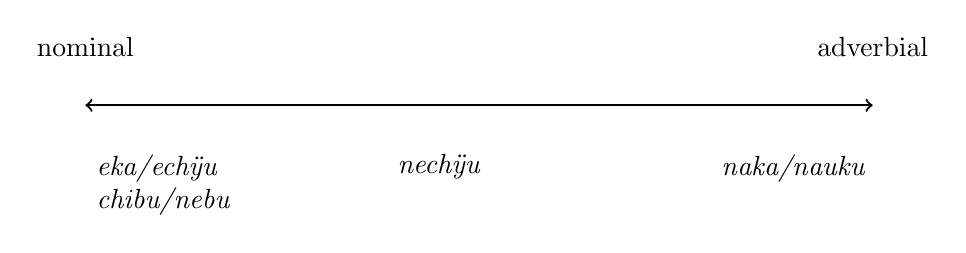
\begin{tikzpicture}
\draw [thick] [<->]  (0,0) -- (10,0);
\node[align=left, above] at (0.0, .5){nominal};%
\node[align=right, above] at (10.0, .5){adverbial};%

\node[align=left, below] at (1.0,-.5)%
    {\textit{eka/echÿu}\\
    \textit{chibu/nebu}};
\node[align=left, below] at (4.5,-.5)%
    {\textit{nechÿu}};
\node[align=left, below] at (9.0,-.5)%
    {\textit{naka/nauku}};
\end{tikzpicture}
\caption{Continuum from more nominal to more adverbial demonstratives}
\label{fig:ContinuumDEMs}
\end{figure}

A few more examples with \textit{nechÿu} follow to illustrate the exophoric use of the demonstrative. In (\getref{ex:demC-1}) and (\getref{ex:demC-5}), it refers to something that is close to the speaker but not within the current interactional space. 

In (\getref{ex:demC-1}), \textit{nechÿu} occurs with the locative-marked NP \textit{nuinekÿyae chubiu bia} ‘at the door of the church’. With this utterance, Miguel described the location of a wooden figure in relation to some other wooden toys that I had placed on my notebook. It is thus a location I had control over, but Miguel did not, thus it was not in his engagement area.\footnote{The engagement area is “the place which is, at moment \textit{t}, the conceived site of a person’s currently dominant manual and attentional engagement” \citep[89]{Enfield2003}.}

\ea\label{ex:demC-1}
\begingl
\glpreamble ja, kaku nechÿu nuinekÿyae chubiu bia\\
\gla ja kaku nechÿu nuinekÿ-yae chÿ-ubiu bia\\
\glb \textsc{afm} exist \textsc{dem}c door-\textsc{loc} 3-house God\\
\glft ‘yes, it is at the door of the church there’
\endgl
\trailingcitation{[mox-e110914l-1.076]}
\xe

In (\getref{ex:demC-5}), Juana tells me about her plans to put a cool box she had just bought in the corridor of her house to sell chicha. We were sitting in the yard, behind the house, the corridor was close to both of us, but not within our (shared) engagement area.

\ea\label{ex:demC-5}
\begingl
\glpreamble nÿsachu netuka nechÿu kureruyae\\
\gla nÿ-sachu nÿ-etuka nechÿu kureru-yae\\
\glb 1\textsc{sg}-want 1\textsc{sg}-put.\textsc{irr} \textsc{dem}c corridor-\textsc{loc}\\
\glft ‘I want to put it in the corridor over there’
\endgl
\trailingcitation{[jxx-e110923l-2.111]}
\xe

The following examples show the anaphoric use of \textit{nechÿu}, i.e. its use to refer back to an antecedent that has either been mentioned by the same speaker or by another person. In (\getref{ex:demC-6}), \textit{nechÿu} refers to the school, \textit{xhikuera}. The sentence comes from Juan C. talking with Miguel about their past and the history of the villages. They had just talked about how much San Miguelito de la Cruz had grown in the preceding decades.

\ea\label{ex:demC-6}
\begingl
\glpreamble nena tanÿma echÿu xhikuera kaku ruschÿ nechÿu, ruschÿ aula metu \\
\gla nena tanÿma echÿu xhikuera kaku ruschÿ nechÿu ruschÿ aula metu\\
\glb like now \textsc{dem}b school exist two \textsc{dem}c two room already\\
\glft ‘it is like with the school now, there are two there, two rooms already’
\endgl
\trailingcitation{[mqx-p110826l.184-186]}
\xe

A similar example is (\getref{ex:nechÿu-1}) by María S., where \textit{nechÿu} anaphorically refers to the basket, which serves as a location for clothes and some food and drink. Note that \textit{-yunu apuke} has an idiomatic meaning ‘walk, go by foot’ (lit.: ‘go ground’) as opposed to ‘go by vehicle’. 


\ea\label{ex:nechÿu-1}
\begingl
\glpreamble apuke niyunupu, apuke nupukenemÿnÿ chupaimÿnÿ nimÿu nechÿu nitapikine\\
\gla apuke ni-yunupu apuke nÿ-upukene-mÿnÿ chupai-mÿnÿ ni-mÿu nechÿu ni-tapiki-ne\\
\glb ground 1\textsc{sg}-go.to ground 1\textsc{sg}-load-\textsc{dim} basket-\textsc{dim} 1\textsc{sg}-clothes \textsc{dem}c 1\textsc{sg}-travel.supplies-\textsc{possd}\\
\glft ‘I walked, walked, with my load, a basket with my clothes in there and my travel supplies’
\endgl
\trailingcitation{[rxx-p181101l-2.036-038]}
\xe


Although \textit{nechÿu} is primarily used to encode spatial relations, the expression \textit{tukiu nechÿu} containing the \isi{source} preposition \textit{tukiu} ‘from’ is often used with a temporal meaning by Juana. This is the case in (\getref{ex:demC-3}), where there is no location in the preceding discourse that could be the referent of \textit{nechÿu}. It is rather the situation itself that is made reference to by the demonstrative.\footnote{As for the sequential \isi{connective} \textit{te}, it sometimes follows \textit{tukiu nechÿu}, but does not seem to be required. There are similar examples without \textit{te}, too.} Other speakers do not use this expression as far as I can tell from the data.

\ea\label{ex:demC-3}
\begingl
\glpreamble tukiu nechÿu te chinekupunubetuji\\
\gla tukiu nechÿu te chi-nekupu-nube-tu-ji\\
\glb from \textsc{dem}c \textsc{seq} 3-see.come-\textsc{pl}-\textsc{iam}-\textsc{rprt}\\
\glft ‘at that point they saw it coming, it is said’
\endgl
\trailingcitation{[jxx-p151016l-2.110]}
\xe


I want to conclude with (\getref{ex:demC-2}), which has the adverb \textit{nauku} ‘there’, the oblique topic pronoun \textit{nebu} and the demonstrative \textit{nechÿu} ‘\textsc{dem}c’. The adverb \textit{nauku} is used to introduce a location into the discourse. In the following clause this location is referred to by the oblique topic pronoun \textit{nebu}, which appears in first position (see \sectref{sec:FocPron}) and once the location is topical,\is{topic} it is taken up again by the demonstrative \textit{nechÿu}. The English translation is ‘there’ in all three cases. The example comes from Juana and is about her plans to move to another part of the city of Santa Cruz, where she was living at that time to care for her grandchildren.

\ea\label{ex:demC-2}
\begingl
\glpreamble biyunupuna nauku, mÿbane la feria, nebu bisemaiku, kakutu nechÿu pero mil \\bolivianos tÿpi entero ubiae\\
\gla bi-yunupuna nauku mÿbane {la feria} nebu bi-semaiku kaku-tu nechÿu pero mil bolivianos tÿpi entero ubiae\\
\glb 1\textsc{pl}-go.back.\textsc{irr} there close {the fair} 3\textsc{obl.top.prn} 1\textsc{pl}-search exist-\textsc{iam} \textsc{dem}c but 1000 bolivianos \textsc{obl} whole house\\
\glft ‘we may go back there, close to the fair, there we looked for it (i.e. a house), there is one now there (offered for rent), but it is (i.e. costs) 1000 bolivianos for the whole house’
\endgl
\trailingcitation{[jxx-p120430l-1.365-369]}
\xe

\is{demonstrative!demonstrative adverb|)}\is{adverb!demonstrative adverb|)}
\is{nominal demonstrative|)}



\largerpage
\subsection{Indefinite pronouns}\label{sec:IndefinitePronouns}
\is{indefinite pronoun|(}

Paunaka uses the question words\is{question word|(} \textit{chija} ‘what, who’ and \textit{juchubu} ‘where’ as indefinite pronouns with the meaning ‘something, someone’ and ‘somewhere’ respectively, see (\getref{ex:chija-INDEF2}) and (\getref{ex:juchubu-INDEF2}).

(\getref{ex:chija-INDEF2}) comes from Juana, who told me about her personal domain to speak Paunaka in the past: the way to the field she walked together with her sister María S.\footnote{This example is also interesting for the use of the verb \textit{-eiku} ‘follow’ as a \isi{preposition} with the meaning ‘along’, see also Footnote \ref{fn:along} in \sectref{sec:SerialVerbs}, and for the verb form \textit{bichujijikÿubÿu} ‘converse walking’ in which the translocative associated motion marker \textit{-CVkÿu} merges with the middle marker \textit{-bu}, but this can be considered an exception.}

\ea\label{ex:chija-INDEF2}
\begingl
\glpreamble chija echÿu bimu cheiku chenekÿ bichujijikÿubÿu bitupubu asaneti\\
\gla chija echÿu bi-imu chÿ-eiku chenekÿ bi-chujiji-kÿu-bu bi-tupu-bu asaneti\\
\glb what \textsc{dem}b 1\textsc{pl}-see 3-along? way 1\textsc{pl}-talk-\textsc{am.conc.tr}-\textsc{mid} 1\textsc{pl}-find-\textsc{mid} field\\
\glft ‘what we saw along the way we talked about walking (until) we reached the field’
\endgl
\trailingcitation{[jxx-p120430l-1.053]}
\xe

(\getref{ex:juchubu-INDEF2}) is also from Juana. She was telling me about the journey of her grandparents back home from Moxos, where they had bought cows.

\ea\label{ex:juchubu-INDEF2}
\begingl
\glpreamble juchubu kaku eka mÿiji tinikujane baka\\
\gla juchubu kaku eka mÿiji ti-niku-jane baka\\
\glb where exist grass 3i-eat-\textsc{distr} cow\\
\glft ‘where there was grass, the cows ate’
\endgl
\trailingcitation{[jxx-p151016l-2.047]}
\xe

It is relatively common cross-linguistically to use “bare interrogatives” as indefinite pronouns, i.e. interrogative pronouns that do not carry any derivational device \citep[170, 174]{Haspelmath2001}. In this scenario, the indefinite use is always secondary to the interrogative use according to \citet[5]{Haspelmath2001}, which is why \textit{chija} and \textit{juchubu} are primarily analysed as question words throughout this work (see \sectref{sec:ContentQuestions}). I also follow \citet{Haspelmath2001} in presenting \textit{juchubu} as an indefinite \textit{pronoun} while it could also be considered an indefinite \textit{adverb}\is{adverb} in a stricter sense.

Use of the indefinite pronouns is relatively rare in Paunaka and they are usually accompanied by a relative clause\is{relative relation} to provide some additional information (see also \sectref{sec:UnmarkedRC} and Footnote \ref{fn:chija} in that section), thus the construction structurally resembles a content question including a question word very much, a sign that use of the question words as indefinite pronouns is not fully grammaticalised.\is{grammaticalisation} However, regarding the use of \textit{chija}, a word of caution is necessary: speakers also use \textit{¿chija?} as a filler in hesitation (‘what was it?’), and it is thus not always clear which function the word has in a specific clause.\is{question word|)} This is the case in (\getref{ex:chija-INDEF1}), which I elicited from María S. in order to speak about Juana, who was making her house in Concepción at that time. Although \textit{chija} could well be an indefinite pronoun here semantically, intonation sets it apart from the rest of the sentence and it is preceded by a false start so it is probably rather to be analysed as a filler here:

\newpage
\ea\label{ex:chija-INDEF1}
\begingl
\glpreamble tisemaiku ti- ¿chija? tisuachi chubiupai\\
\gla ti-semaiku ti- chija ti-isua-chi chÿ-ubiupai\\
\glb 3i-search 3i- what 3i-weed.\textsc{irr}-3 3-plot\\
\glft ‘she is looking for ¿what was it? someone to weed her plot’
\endgl
\trailingcitation{[rxx-e120511l.047]}
\xe

In the other examples I give here \textit{chija} is not set apart from the rest of the sentence by intonation, pauses or false starts, thus I am fairly confident that we are dealing with the indefinite pronoun rather than with any other use of the word. There may be more examples of the indefinite use that I have mistakenly taken to represent the use as filler.

(\getref{ex:chija-INDEF3}) includes the negative particle \textit{kuina}. It is taken from María S.’s story about the two hunters who meet the devil in the woods. One man feeds the devil with the meat they hunted, but the devil does not fill up, thus finally, the man has to admit:

\ea\label{ex:chija-INDEF3}
\begingl
\glpreamble “kuinabutu chija nenikapi”\\
\gla kuina-bu-tu chija nÿ-nika-pi\\
\glb \textsc{neg}-\textsc{dsc} what 1\textsc{sg}-feed.\textsc{irr}-2\textsc{sg}\\
\glft ‘“there isn’t anything left that I could give you to eat”’
\endgl
\trailingcitation{[rxx-n120511l-2.45-46]}
\xe


The next example also contains \textit{kuina} and comes from the recordings made by Riester. Juan Ch. talks about his life in Retiro. 
%-kine = emphatic here!

\ea\label{ex:RCchija2}
\begingl
\glpreamble kuina chija baejumikine, micha bubiu nakaja\\
\gla kuina chija bi-a-ejumi-kene micha bi-ub-i-u naka-ja\\
\glb \textsc{neg} what 1\textsc{pl}-\textsc{irr}-remember-\textsc{emph}2 good 1\textsc{pl}-be-\textsc{subord}-\textsc{real} here-\textsc{emph}1\\
\glft ‘there is nothing to think about (i.e. complain about?), our living here is good’
\endgl
\trailingcitation{[nxx-p630101g-1.175]}
\xe

It is possible that \textit{chija} needs to be accompanied obligatorily by further material to be made more precise, this would explain why Juana adds \textit{echÿu} in the following example. She is making a statement here about me getting my stuff ready to travel back to Germany.

\newpage

\ea\label{ex:chija-INDEF4}
\begingl
\glpreamble komoraubinatu [...] masa arbiraubina chija echÿu\\
\gla komorau-bi-ina-tu masa arbirau-bi-ina chija echÿu\\
\glb accomodate-2\textsc{sg}-\textsc{irr.nv}-\textsc{iam} lest forget-2\textsc{sg}-\textsc{irr.nv} what \textsc{dem}b\\
\glft ‘you have to arrange (your stuff) now lest you forget something’
\endgl
\trailingcitation{[jxx-p120515l-2.276-278]}
\xe

%indirect question: ¿chijakena tububuichu eka ubiae?, kuina bichupa chija tanaubanechÿ eka ubiae, rxx-e201231f.38

In contrast, \textit{juchubu} ‘where’ can stand on its own in indefinite use, although this is rare. An example of its free use is (\getref{ex:juchubu-INDEF1}) from Juana talking about a house they want to pay with a credit.

\ea\label{ex:juchubu-INDEF1}
\begingl
\glpreamble i kue biyunatu juchubu tipuabinube tÿmuepupunuku\\
\gla i kue bi-yuna-tu juchubu ti-pua-bi-nube tÿmue-pupunuku\\
\glb and if 1\textsc{pl}-go.\textsc{irr}-\textsc{iam} where 3i-give.\textsc{irr}-1\textsc{pl}-\textsc{pl} money-\textsc{reg}\\
\glft ‘and if we go somewhere else, they give us the money back’
\endgl
\trailingcitation{[jxx-p120430l-1.388]}
\xe

Usually, however, \textit{juchubu} is also accompanied by a relative clause to specify the nature of the indefinite place as in (\getref{ex:RCwhere2}), where María S. tells Swintha about how tortoises lay their eggs.

\ea\label{ex:RCwhere2}
\begingl
\glpreamble juchubu tisachu tisukupunuka, naukuku tisekumÿnÿ epenue, tisukuka nechÿu, depue tiyunuka\\
\gla juchubu ti-sachu ti-suku-punuka nauku-uku ti-seku-mÿnÿ epenue ti-suku-uka nechÿu depue ti-yunuka\\
\glb where 3i-want 3i-lay.egg-\textsc{reg.irr} there-\textsc{add} 3i-dig.hole-\textsc{dim} hole 3i-lay.egg-\textsc{add.irr} \textsc{dem}c afterwards 3i-go.on.\textsc{irr}\\
\glft ‘where it (the tortoise) wants to lay eggs again, there it also digs a little hole to lay eggs again there, then it will go on’
\endgl
\trailingcitation{[rxx-e121128s-1.090]}
\xe

Just like in questions, \textit{juchubu} can be followed by a \isi{deranked verb} as in (\getref{ex:go-search-field-1}), elicited from Miguel.

\ea\label{ex:go-search-field-1}
\begingl
\glpreamble ukuine niyunu nisemaikupa juchubu nanaia nisaneina\\
\gla ukuine ni-yunu ni-semaiku-pa juchubu nÿ-ana-i-a ni-sane-ina\\
\glb yesterday 1\textsc{sg}-go 1\textsc{sg}-search-\textsc{dloc.irr} where 1\textsc{sg}-make-\textsc{subord}-\textsc{irr} 1\textsc{sg}-field-\textsc{irr.nv}\\
\glft ‘yesterday I went to look for somewhere to make my future field’
\endgl
\trailingcitation{[mxx-e160811sd.152]}
\xe % -> also in chapter adverbial clauses!

It is unclear at the moment which conditions favour the use of a \isi{deranked verb}, this must remain a question for further research for the time being.

\is{indefinite pronoun|)}
\is{pronoun|)}

%i tikechunubetu: eyuna n- esamaikupa juchubu ubiuyae, mxx-p110825l.051-052

%bi- bisemaiku otra juchubu bitibuia, mqx-p110826l.016

%temporal: sí aa kuina naichunabane juchubu u tu tijaibane kapunu piesta, sí, aa, antes no sabía qué día vino una fiesta, rxx-p181101l-2.013 -> indirect question?

The following section deals with adjectives, numerals, and quantifiers.



